\newcounter{english}
\documentclass{article}

% packages
\usepackage{amsmath, amsthm, thmtools, amsfonts, amssymb, luacode, catchfile, tikzducks, hyperref, ifthen}
\ifcsname c@kobocompile\endcsname
	\usepackage[a5paper, total={1072pt, 1448pt}, margin=10pt, includeheadfoot]{geometry} % set page margins
\else
	\usepackage[a4paper, margin=50pt, includeheadfoot]{geometry}
\fi
\usepackage[shortlabels]{enumitem}
\usepackage[skip=3pt, indent=0pt]{parskip}

% language
\usepackage[bidi=basic, layout=tabular, provide=*]{babel}
\ifcsname c@english\endcsname
	\babelprovide[main, import]{english}
\else
	\babelprovide[main, import]{hebrew}
	\babelprovide{rl}
\fi
%\babelfont{rm}{Libertinus Serif}
\babelfont{rm}[Renderer=Harfbuzz]{Libertinus Serif}
\babelfont{sf}{Libertinus Sans}
\babelfont{tt}{Libertinus Mono}

% style
\AddToHook{cmd/section/before}{\clearpage}	% Add line break before section
\linespread{1.3}
\setcounter{secnumdepth}{0}		% Remove default number tags from sections, this won't do well with theorems
\AtBeginDocument{\setlength{\belowdisplayskip}{3pt}}
\AtBeginDocument{\setlength{\abovedisplayskip}{3pt}}
\graphicspath{ {../images/} }

% operators
\DeclareMathOperator\cis{cis}
\DeclareMathOperator\Sp{Sp}
\DeclareMathOperator\tr{tr}
\DeclareMathOperator\im{Im}
\DeclareMathOperator\re{Re}
\DeclareMathOperator\diag{diag}
\DeclareMathOperator*\lowlim{\underline{lim}}
\DeclareMathOperator*\uplim{\overline{lim}}
\DeclareMathOperator\rng{rng}
\DeclareMathOperator\Sym{Sym}
\DeclareMathOperator\Arg{Arg}
\DeclareMathOperator\Log{Log}
\DeclareMathOperator\dom{dom}
\DeclareMathOperator\supp{Supp}
\DeclareMathOperator\var{Var}
\DeclareMathOperator\cov{Cov}

% commands
%\renewcommand\qedsymbol{\textbf{מש''ל}}
%\renewcommand\qedsymbol{\fbox{\emoji{lizard}}}
\newcommand{\Aa}[0]{\mathcal{A}}
\newcommand{\Bb}[0]{\mathcal{B}}
\newcommand{\CC}[0]{\mathbb{C}}
\newcommand{\Cc}[0]{\mathcal{C}}
\newcommand{\EE}[0]{\mathbb{E}}
\newcommand{\FF}[0]{\mathbb{F}}
\newcommand{\Ff}[0]{\mathcal{F}}
\newcommand{\Ii}[0]{\mathcal{I}}
\newcommand{\Gg}[0]{\mathcal{G}}
\newcommand{\Ll}[0]{\mathcal{L}}
\newcommand{\Mm}[0]{\mathcal{M}}
\newcommand{\NN}[0]{\mathbb{N}}
\newcommand{\Nn}[0]{\mathcal{N}}
\newcommand{\PP}[0]{\mathbb{P}}
\newcommand{\Pp}[0]{\mathcal{P}}
\newcommand{\QQ}[0]{\mathbb{Q}}
\newcommand{\RR}[0]{\mathbb{R}}
\newcommand{\Rr}[0]{\mathcal{R}}
\newcommand{\Ss}[0]{\mathcal{S}}
\newcommand{\TT}[0]{\mathbb{T}}
\newcommand{\Uu}[0]{\mathcal{U}}
\newcommand{\Vv}[0]{\mathcal{V}}
\newcommand{\Ww}[0]{\mathcal{W}}
\newcommand{\ZZ}[0]{\mathbb{Z}}
\newcommand{\acts}[0]{\circlearrowright}
\newcommand{\explain}[2] {
	\begin{flalign*}
		 && \text{#2} && \text{#1}
	\end{flalign*}
}
\newcommand{\maketitleprint}[0]{ \begin{center}
	%\begin{tikzpicture}[scale=3]
	%	\duck[graduate=gray!20!black, tassel=red!70!black]
	%\end{tikzpicture}	
	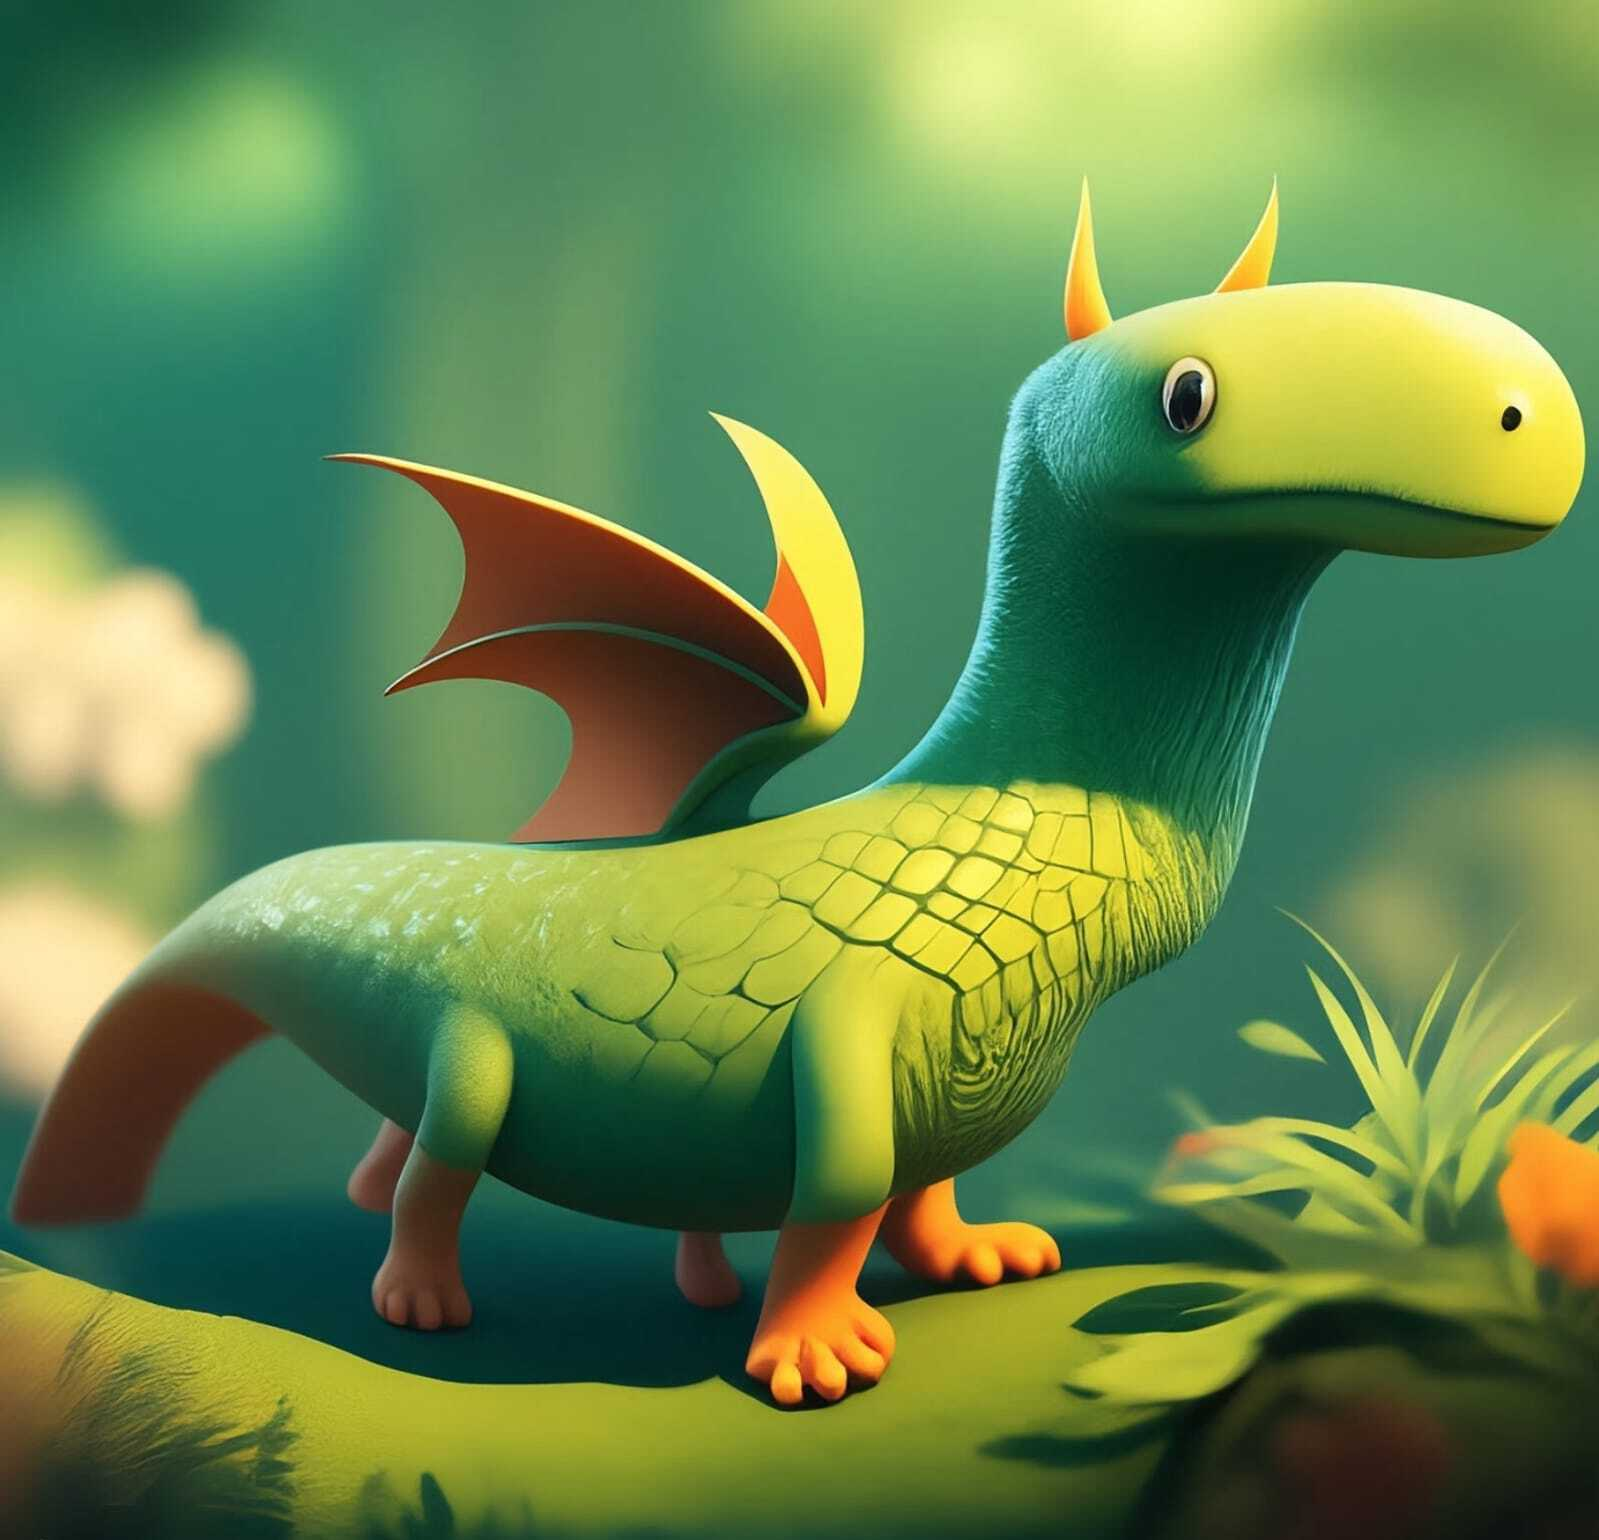
\includegraphics[width=6cm]{cover}
\end{center}
}

% theorem commands
\newtheoremstyle{c_remark}
	{}	% Space above
	{}	% Space below
	{}% Body font
	{}	% Indent amount
	{\bfseries}	% Theorem head font
	{}	% Punctuation after theorem head
	{.5em}	% Space after theorem head
	{\thmname{#1}\thmnumber{ #2}\thmnote{ \normalfont{\text{(#3)}}}}	% head content
\newtheoremstyle{c_definition}
	{3pt}	% Space above
	{3pt}	% Space below
	{}% Body font
	{}	% Indent amount
	{\bfseries}	% Theorem head font
	{}	% Punctuation after theorem head
	{.5em}	% Space after theorem head
	{\thmname{#1}\thmnumber{ #2}\thmnote{ \normalfont{\text{(#3)}}}}	% head content
\newtheoremstyle{c_plain}
	{3pt}	% Space above
	{3pt}	% Space below
	{\itshape}% Body font
	{}	% Indent amount
	{\bfseries}	% Theorem head font
	{}	% Punctuation after theorem head
	{.5em}	% Space after theorem head
	{\thmname{#1}\thmnumber{ #2}\thmnote{ \text{(#3)}}}	% head content

\ifcsname c@english\endcsname
	\theoremstyle{plain}
	\newtheorem{theorem}{Theorem}[section]
	\newtheorem{lemma}[theorem]{Lemma}
	\newtheorem{proposition}[theorem]{Proposition}
	\newtheorem*{proposition*}{Proposition}
	%\newtheorem{corollary}[theorem]{אין חלופה עברית}

	\theoremstyle{definition}
	\newtheorem{definition}[theorem]{Definition}
	\newtheorem*{definition*}{Definition}
	\newtheorem{example}{Example}[section]
	\newtheorem{exercise}{Exercise}[section]

	\theoremstyle{remark}
	\newtheorem*{remark}{Remark}
	\newtheorem*{solution}{Solution}
	\newtheorem{conclusion}[theorem]{Conclusion}
	\newtheorem{notation}[theorem]{Notation}
\else
	\theoremstyle{c_plain}
	\newtheorem{theorem}{משפט}[section]
	\newtheorem{lemma}[theorem]{למה}
	\newtheorem{proposition}[theorem]{טענה}
	\newtheorem*{proposition*}{טענה}
	%\newtheorem{corollary}[theorem]{אין חלופה עברית}

	\theoremstyle{c_definition}
	\newtheorem{definition}[theorem]{הגדרה}
	\newtheorem*{definition*}{הגדרה}
	\newtheorem{example}{דוגמה}[section]
	\newtheorem{exercise}{תרגיל}[section]

	\theoremstyle{c_remark}
	\newtheorem*{remark}{הערה}
	\newtheorem*{solution}{פתרון}
	\newtheorem{conclusion}[theorem]{מסקנה}
	\newtheorem{notation}[theorem]{סימון}
\fi

% Questions related commands
\newcounter{question}
\setcounter{question}{1}
\newcounter{sub_question}
\setcounter{sub_question}{1}

\ifcsname c@english\endcsname
	\newcommand{\question}[1][0]{
		\ifthenelse{#1 = 0}{}{\setcounter{question}{#1}}
		\section{Question \arabic{question}}
		\addtocounter{question}{1}
		\setcounter{sub_question}{1}
	}

	\newcommand{\subquestion}[1][0]{
		\ifthenelse{#1 = 0}{}{\setcounter{sub_question}{#1}}
		\subsection{Part \alph{sub_question}}
		\addtocounter{sub_question}{1}
	}
\else
	\newcommand{\question}[1][0]{
		\ifthenelse{#1 = 0}{}{\setcounter{question}{#1}}
		\section{שאלה \arabic{question}}
		\addtocounter{question}{1}
		\setcounter{sub_question}{1}
	}

	\newcommand{\subquestion}[1][0]{
		\ifthenelse{#1 = 0}{}{\setcounter{sub_question}{#1}}
		\subsection{סעיף \localecounter{letters.gershayim}{sub_question}}
		\addtocounter{sub_question}{1}
	}
\fi

% import lua and start of document
\directlua{common = require ('../common')}

\GetEnv{AUTHOR}

% headers
\author{\AUTHOR}
\date\today

\title{Exercise 9 Answer Sheet --- Logic Theory (2), 80424}

\DeclareMathOperator{\PA}{PA}
\DeclareMathOperator{\Coll}{Coll}
\DeclareMathOperator{\Ind}{Ind}
\DeclareMathOperator{\Sat}{Sat}

\begin{document}
\maketitle
\maketitleprint[yellow]

\question{}
\subquestion{}
We will show that the set,
\[
	H
	= \{ e \in \NN \mid (e, 0) \in \dom U \}
\]
is recursively-enumerable but not recursive.
\begin{proof}
	$H$ is $\Sigma_1^0$ by the definition of $U$, implies that it is recursively-enumerable, then it is sufficient to show that it is not recursive.
	Let $f : \NN \to \NN$ be the function defined by,
	\[
		f(x) = x
	.\]
	This is indeed a recursive function (even primitive-recursive), and for every $e \in D$, when $D = \{ e \in \NN \mid (e, e) \in \dom U \}$, we get $f(e) = e \in H$, as $e$ witnessing bound larger than $0$.
	It follows that $f$ is a recursive reduction of $D$ to $H$ and implies that $H$ is not recursive.
\end{proof}

\subquestion{}
We will conclude that $H^C = \NN \setminus H$ is not recursively-enumerable.
\begin{proof}
	$H$ is a relation, meaning that if it were to be $\Pi_1^0$ it would be $\Delta_1^0$ and recursive.
	If $H^C$ is recursively-enumerable then $H^C = \{ e \in \NN \mid (e, 0) \in \dom(\lnot U) \}$ is $\Sigma_1^0$, and implying by negation that $H = \lnot H^C$ (in the sense of relations) is $\Pi_1^0$.
	But $H$ is recursively-enumerable and $\Sigma_1^0$, meaning that it is indeed $\Delta_1^0$, in contradiction to its being not recursive.
\end{proof}

\subquestion{}
Let us define the set,
\[
	T = \{ e \in \NN \mid \{ x \mid (e, x) \in \dom U \} = \NN \}
\]
We will show that $T$ is not recursively-enumerable.
\begin{proof}
	We assume in contradiction that $T$ is recursively-enumerable. \\
	By the equivalence to recursively-enumerable functions proposition we can assume that there is a function $f : \NN \to \NN$ such that $f$ is primitive-recursive and $T = \{ f(x) \mid x \in \NN \}$.
	Let us define $g : \NN^2 \to \NN$ by,
	\[
		g(n, x) = U(f(n), x) + 1
	\]
	$g$ is indeed total recursive function as $U$ is recursive and $f$ is total such that $U(f(n), \cdot)$ is total recursive function.
	$h(x) = g(x, x) + 1 = U(f(x), x) + 1$ is a total recursive function.
	This means that $\# h \in T$, and there is $m \in \NN$ such that $f(m) = \# h$.
	\[
		h(m)
		= U(f(m), m) + 1
		= U(\# h, m) + 1
		= h(m) + 1
	\]
	This is contradiction by diagonalization.
\end{proof}

\subquestion{}
We will show that $T^C = \NN \setminus T$ is not recursively-enumerable.
\begin{proof}
	We will find a function that maps the code of a recursive function to the code of a constant function to return the value at zero of the initial function.
	In other words, we want a function $g$ such that,
	\[
		U(g(e), x)
		= U(e, 0)
	\]
	Let us define,
	\[
		F(e, x)
		= U(e, 0)
	\]
	By the fixed point theorem there exists $g$ recursive such that,
	\[
		U(g(e), x)
		= F(e, x)
		= U(e, 0)
	\]
	Then $g$ is exactly the function we wanted.

	For any $e \in H$ we get some total recursive function code, and in particular $g(e) \in T$.
	For $e \notin H \iff e \in H^C$ it follows that $g(e)$ is not defined for any $x \in \NN$, in particular $g(e) \in T^C$.
	We conclude that $g^{-1}(T^C) = H^C$, if we assume in contradiction that $T^C$ is recursively-enumerable then by the pre-image theorem it follows that $H^C$ is recursively-enumerable,
	a contradiction to the previous parts conclusion.
\end{proof}

\question{}
We will show that any infinite recursively-enumerable set contains an infinite recursive subset.
\begin{proof}
	Let $X$ be some recursively-enumerable set.
	Let $f : \NN \to \NN$ be a total primitive-recursive function such that $X = f(\NN)$.
	We saw that $\max$ is primitive-recursive, then,
	\[
		g(x) = \max \{ f(n) \mid n < x \}
	\]
	is primitive-recursive as well.
	Note that $f$ is unbounded, therefore $g$ is unbounded as well.
	We define $h : \NN \to \{ 0, 1\}$ by,
	\[
		h(x)
		= \begin{cases}
			1 & g(x) = f(x) \\
			0 & \text{otherwise}
		\end{cases}
	\]
	This is primitive-recursive function as the cases operation is primitive, and $h = \chi_Y$ for $Y \subseteq X$ recursive as we wanted.
\end{proof}

\question{}
We define the sets $A, B \subseteq \NN$ as recursively-separated if there is some recursive set $C \subseteq \NN$ such that $A \subseteq C$ and $B \cap C = \emptyset$. \\
We will find an example of two disjoint recursively-enumerable subsets of $\NN$ which cannot be recursively-separated.
\begin{solution}
	Let $f : \NN \to \NN$ be the function such that $f(\NN) = H$ from the first question.
	We define $A = \{ f(2n) \mid n \in \NN \}$ and $B = \{ f(2n + 1) \mid n \in \NN \}$, these are clearly recursively-enumerable but not recursive.
	We also see that $A \cap B = \emptyset$ directly by definition.

	Let us assume in contradiction that there is a recursive $C \subseteq \NN$ such that $A \subseteq C$ and $B \cap C = \emptyset$.
	But the set of recursive functions $R$ is recursive and the reduction of recursive function is recursive, then $R \cap C = A$ is recursive, in contradiction to question 1.

	Note that $f$ might not be injective, meaning that $A \cap B$ might not be null.
	To solve this, we define new recursive function, $g : \NN \to \NN$ by,
	\[
		g(n)
		= \min\{ f(k) \mid i > n, f(k) > g(n - 1) \}
	\]
	This function is recursive directly as the minimization of recursive function $f$.
	We also derive from $|\im f| = \omega$ that $g$ is total and that $\im g \subseteq \im f$.
	In particular, using $g$ instead of $f$ we get $A \cap B = \emptyset$ as wished.
\end{solution}

\end{document}
